\lstset{frame=tb,
	language=C++,
	aboveskip=3mm,
	belowskip=3mm,
	showstringspaces=false,
	columns=flexible,
	basicstyle={\small\ttfamily},
	numbers=none,
	numberstyle=\tiny,
	breaklines=true,
	breakatwhitespace=true,
	tabsize=3}

\chapter{Verificarea formală a problemei}

\section{Implementarea algoritmului}
    Implementarea algoritmului propriu-zis care rezolvă problema a fost primul și cel mai ușor pas.\par
    Am început prin crearea unei bucle care la fiecare pas alegea bancnota optimă, o adăuga în secvența de 
    bancnote considerată soluție și o scădea din sumă, fiind un algoritm tipic metodei Greedy.
    \begin{lstlisting}
    var rest:= sum;
    solution:= [0, 0, 0, 0, 0, 0];
    while (0 < rest)
        decreases rest 
        {
        index:= maxBanknote(rest);
        var banknote:= power(2, index);
        solution:= addValueToIndex(solution,1,index);
        rest:= rest - banknote;
    }
    \end{lstlisting}

    Acest algoritm era suficient pentru a rezolva problema, dar nu era suficient pentru a demonstra că soluția produsă este optimă.\par
    Considerăm o soluție optimă soluția de cost minim, costul fiind numărul de bancnote.
    
\section{Demonstrarea optimalității}
    \subsection{Schema verificării}
    \vspace{1cm}
    \begin{center}
        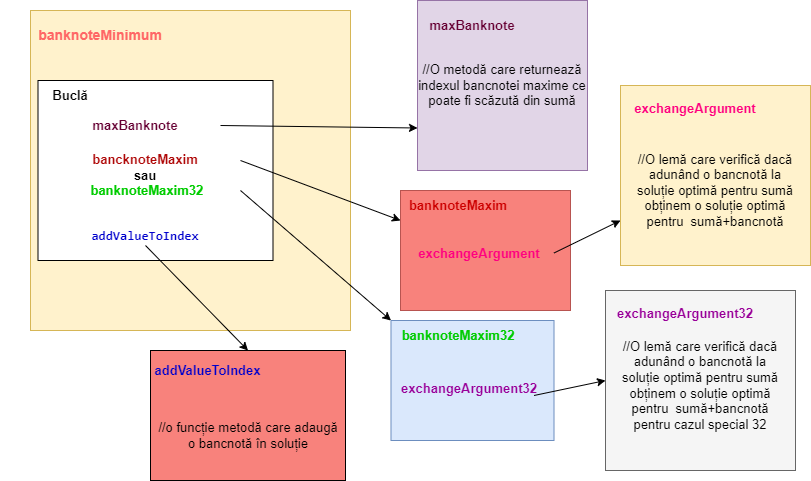
\includegraphics[width=1.0\textwidth]{verification_schema.png}\par
    \end{center}
    În schema de mai sus am exemplificat modul în care funcțiile, lemele și metodele se apelează una pe cealaltă pentru a demonstra faptul că soluția găsită este soluție optimă.\par

    \subsection{Condiții ca o soluția finală să fie optimă}
    $\bullet$ Pentru a avea o soluție optimă trebuie să avem o soluție validă (cu 6 elemente), care produce suma corectă
     și care are costul cel mai mic.\par
    $\bullet$ Pentru a avea o soluție optimă finală, pe parcursul construirii soluției, în buclă, trebuie menținută proprietatea
     de a alege soluția optimă locală pentru rest, iar suma soluțiilor optime locale să fie soluție optimă pentru sumă.\par
    $\bullet$ Soluția formată dintr-o bancnotă, cea aleasă în iterația curentă, produce o soluție optimă pentru suma 
    de valoare bancnotă, asigurând faptul că avem o soluție optimă locală.\par
    $\bullet$ O soluție optimă pentru suma $x$, adunată cu o soluție optimă pentru suma $y$ creează o soluție optimă pentru suma $x+y$, 
    asigurând faptul că suma soluțiilor locale creează soluția finală optimă.\par
    
\section{Pașii verificării}
    \subsection{banknoteMinimum}
    Am implementat algoritmul Greedy care rezolva Problema Bancnotelor cu bancnote puteri ale lui 2, 
    apoi am adăugat treptat condițiile care garantează că soluția găsită este soluție optimă.\par
    \begin{lstlisting}
    method banknoteMinimum(sum: int) returns(solution: seq < int > )
        requires sum >= 0
        ensures isValidSolution(solution)
        ensures isSolution(solution, sum)
        ensures isOptimalSolution(solution, sum) 
    {
        var rest:= sum;
        solution:= [0, 0, 0, 0, 0, 0];
        var index:= 0;
        assert isOptimalSolution(solution, sum - rest);
        while (0 < rest)
            invariant 0 <= rest <= sum
            invariant isValidSolution(solution)
            invariant addOptimRestEqualsOptimSum(rest, sum, solution)
            decreases rest 
        {
            index:= maxBanknote(rest);
            var banknote:= power(2, index);
            if (index != 5) 
            {
                banknoteMaxim(rest, sum, solution, index);
            } 
            else 
            {
                banknoteMaxim32(rest, sum, solution);
            }
            solution:= addValueToIndex(solution,1,index);
            rest:= rest - banknote;
        }
    }
    \end{lstlisting}
    \subsection{maxBanknote}
    Pentru a alege bancnota cea mai mare am creat funcția maxBanknote.\par
    \begin{lstlisting}
      method maxBanknote(sum: int) returns(index: int)
        requires sum > 0
        ensures 0 <= index <= 5
        ensures 0 <= power(2, index) <= sum
        ensures(index != 5 && power(2, index + 1) > sum) || index == 5 
      {
        index:= 5;
        if (power(2, index) > sum) 
        {
          assert power(2, index + 1) > sum;
          while (power(2, index) > sum && index > 0)
            invariant power(2, index + 1) > sum 
            {
              index:= index - 1;
              assert power(2, index + 1) > sum;
            }
        } 
          else 
        {
          //we know the index is 5
          assert index == 5;
        }
      }
    \end{lstlisting}


    \subsection{banknoteMaxim}
    \begin{lstlisting}
    lemma banknoteMaxim(rest: int, sum: int, finalSolution: seq < int > , index: int)
        requires 0 <= index <= 4
        requires power(2, index) <= rest < power(2, index + 1)
        requires isValidSolution(finalSolution)
        requires addOptimRestEqualsOptimSum(rest, sum, finalSolution)
        ensures addOptimRestEqualsOptimSum(rest - power(2, index), sum, finalSolution[index:= finalSolution[index] + 1]) 
    {
    var banknote:= power(2, index);
    forall currentSolution | isValidSolution(currentSolution) && isOptimalSolution(currentSolution, rest - banknote)
        ensures isOptimalSolution(solutionsSum(solutionsSum(currentSolution, finalSolution), [0, 0, 0, 0, 0, 0][index:= 1]), sum) 
    {
        assert isSolution(currentSolution[index:= currentSolution[index] + 1], rest);
        exchangeArgument(rest, currentSolution, index);
    }
    assert forall currentSolution::isValidSolution(currentSolution) && isOptimalSolution(currentSolution, rest - banknote) ==> isOptimalSolution(solutionsSum(solutionsSum(currentSolution, finalSolution), [0, 0, 0, 0, 0, 0][index:= 1]), sum);
    }
    \end{lstlisting}

    \subsection{exchangeArgument}
    \begin{lstlisting}
        lemma exchangeArgument(rest: int, currentSolution: seq < int > , index: int)
            requires 0 <= index <= 4
            requires power(2, index) <= rest < power(2, index + 1)
            requires isValidSolution(currentSolution)
            requires isOptimalSolution(currentSolution, rest - power(2, index))
            ensures isOptimalSolution(currentSolution[index:= currentSolution[index] + 1], rest) 
        {
            var banknote:= power(2, index);
            var solution:= currentSolution[index:= currentSolution[index] + 1];
            assert isValidSolution(solution);
            assert isSolution(solution, rest);
            var i:= index;
            if (!isOptimalSolution(solution, rest)) 
            {
            var optimalSolution:| isValidSolution(optimalSolution) && isSolution(optimalSolution, rest) &&
                isOptimalSolution(optimalSolution, rest) && cost(optimalSolution) < cost(solution);

            assert cost(solution) == cost(currentSolution) + 1;
            assert isOptimalSolution(optimalSolution, rest);

            if (optimalSolution[index] -1 >= 0) 
            {
                assert optimalSolution[index]-1 >= 0;
                var betterSolution:= addValueToIndex(optimalSolution,-1,index);
                assert isSolution(betterSolution, rest - banknote);
                assert cost(betterSolution) == cost(optimalSolution) - 1;
                assert cost(optimalSolution) - 1 < cost(currentSolution);
                assert false;
            } 
            else 
            {
                while (0 < i)
                invariant 0 <= i <= index
                invariant forall x::index >= x >= i ==> optimalSolution[x] <= 1 
                {
                i:= i - 1;
                assert isOptimalSolution(optimalSolution, rest);
                if (optimalSolution[i] > 1) 
                {
                    var optimalSolution' := optimalSolution[i:=optimalSolution[i]-2];
                    optimalSolution' := optimalSolution' [i + 1:= optimalSolution'[i+1]+1];
                    assert isSolution(optimalSolution', rest);
                    assert cost(optimalSolution') == cost(optimalSolution) - 1;
                    assert cost(optimalSolution') < cost(optimalSolution);
                    assert false;
                }
                }
                assert solutionElementsSum(optimalSolution) <= banknote - 1; assert rest >= banknote; assert solutionElementsSum(optimalSolution) <= rest - 1; assert isOptimalSolution(optimalSolution, rest); assert false;
            }
            }
        }
    \end{lstlisting}

    \subsection{addValueToIndex}
    \begin{lstlisting}
        function method addValueToIndex(solution: seq<int>, value: int, index: int): seq<int>
            requires 0 <= index <= 5
            requires isValidSolution(solution)
            requires solution[index] + value >= 0
            ensures isValidSolution(solution)
            ensures solutionElementsSum(solution) + value*power(2, index) == solutionElementsSum(solution[index:=solution[index]+value])
        {
        solution[index:= solution[index] + value]
        }
    \end{lstlisting}

    
    \subsection{Ultimul pas}
    În final, am descoperit că pentru bancnota 32 am nevoie de o verificare diferită.\par
    Voi descrie ulterior cum am tratat acest caz.\par
    -de ce trebuie abordata diferit- 
    
    
    
\section{Problema bancnotei nemărginite superior, 32}

\subsection{Cum se tratează separat cazul 32}

\subsection{banknoteMaxim32}
\begin{lstlisting}
lemma banknoteMaxim32(rest: int, sum: int, finalSolution: seq < int > )
  requires rest >= 32
  requires isValidSolution(finalSolution)
  requires addOptimRestEqualsOptimSum(rest, sum, finalSolution)
  ensures addOptimRestEqualsOptimSum(rest - 32, sum, solutionsSum(finalSolution, [0, 0, 0, 0, 0, 1])) 
{
  forall currentSolution | isValidSolution(currentSolution) && isSolution(currentSolution, rest - 32)
    ensures isSolution(solutionsSum(solutionsSum(finalSolution, currentSolution), [0, 0, 0, 0, 0, 1]), sum) 
  {
    assert isSolution(solutionsSum(currentSolution, [0, 0, 0, 0, 0, 1]), rest);
  }

  forall currentSolution | isValidSolution(currentSolution) && isOptimalSolution(currentSolution, rest - 32)
    ensures isOptimalSolution(solutionsSum(solutionsSum(finalSolution, currentSolution), [0, 0, 0, 0, 0, 1]), sum)
  {
    forall someSolution | isValidSolution(someSolution) && isSolution(someSolution, sum)
      ensures cost(someSolution) >= cost(solutionsSum(solutionsSum(finalSolution, currentSolution), [0, 0, 0, 0, 0, 1])) 
    {
      currentSolutionHasCostMin(rest, sum, currentSolution);
    }
  }
}
\end{lstlisting}

\subsection{currentSolutionHasCostMin}
\begin{lstlisting}
    lemma currentSolutionHasCostMin(rest: int, sum: int, solution: seq < int > )
  requires isValidSolution(solution)
  requires rest >= 32
  requires isSolution(solution, rest - 32)
  requires isOptimalSolution(solution, rest - 32)
  ensures isOptimalSolution(solutionsSum(solution, [0, 0, 0, 0, 0, 1]), rest) 
{
  forall someSolution | isValidSolution(someSolution) && isSolution(someSolution, rest)
    ensures cost(someSolution) >= cost(solutionsSum(solution, [0, 0, 0, 0, 0, 1])) 
  {
    exchangeArgument32(rest, sum, someSolution, solution);
  }
}

\end{lstlisting}


\subsection{exchangeArgument32}
\begin{lstlisting}
    
lemma exchangeArgument32(rest: int, sum: int, currentSolution: seq < int > , optimalSolution: seq < int > )
    requires 32 <= rest
    requires isValidSolution(optimalSolution)
    requires isOptimalSolution(optimalSolution, rest - 32)
    ensures isOptimalSolution(optimalSolution[5:= optimalSolution[5] + 1], rest) 
{
    var solution:= optimalSolution[5:= optimalSolution[5] + 1];
    var i:= 4;
    if (!isOptimalSolution(solution, rest)) 
    {
        if (optimalSolution[i] > 1) 
        {
            var solution:= optimalSolution[i:= optimalSolution[i] - 2];
            solution:= solution[i + 1:= solution[i + 1] + 1];
            assert isSolution(solution, rest - 32);
            assert cost(solution) == cost(optimalSolution) - 1;
            assert cost(optimalSolution) - 1 < cost(solution);
            assert false;
        } 
        else
        {
            while (0 < i)
                invariant 0 <= i <= 4
                invariant forall index::4 >= index >= i ==> optimalSolution[index] <= 1 
            {
                i:= i - 1;
                if (optimalSolution[i] > 1) 
                {
                    var solution:= optimalSolution[i:= optimalSolution[i] - 2];
                    solution:= solution[i + 1:= solution[i + 1] + 1];
                    assert isSolution(solution, rest - 32);
                    assert cost(solution) == cost(optimalSolution) - 1;
                    assert cost(optimalSolution) - 1 < cost(solution);
                    assert false;
                }
                assert optimalSolution[i] <= 1;
            }
            assert solutionElementsSum(optimalSolution) <= rest - 1;
            assert isOptimalSolution(solution, rest);
            assert false;
        }
    }
}

\end{lstlisting}

